%% LyX 2.3.4.2 created this file.  For more info, see http://www.lyx.org/.
%% Do not edit unless you really know what you are doing.
\documentclass[ruled]{article}
\usepackage{courier}
\usepackage[T1]{fontenc}
\usepackage[latin9]{inputenc}
\usepackage[letterpaper]{geometry}
\geometry{verbose}
\usepackage{color}
\usepackage{algorithm2e}
\usepackage{amsmath}
\usepackage{amssymb}
\usepackage{graphicx}
\usepackage[unicode=true,
 bookmarks=false,
 breaklinks=false,pdfborder={0 0 1},backref=section,colorlinks=true]
 {hyperref}
 
 \usepackage{parskip}
\setlength{\parindent}{0pt}

\usepackage{graphicx}
\usepackage{fancyhdr}
\usepackage[dvipsnames]{xcolor}
\usepackage{ifthen}
\usepackage{titlesec}

\titleformat{\section}
{\color{RoyalPurple}\normalfont\Large\bfseries}
{\color{RoyalPurple}\thesection}{1em}{}

\titleformat{\subsection}
{\color{RoyalPurple}\normalfont\large\bfseries}
{\color{RoyalPurple}\thesubsection}{1em}{}

\makeatletter

%%%%%%%%%%%%%%%%%%%%%%%%%%%%%% LyX specific LaTeX commands.
\providecommand{\LyX}{\texorpdfstring%
  {L\kern-.1667em\lower.25em\hbox{Y}\kern-.125emX\@}
  {LyX}}
%% Special footnote code from the package 'stblftnt.sty'
%% Author: Robin Fairbairns -- Last revised Dec 13 1996
\let\SF@@footnote\footnote
\def\footnote{\ifx\protect\@typeset@protect
    \expandafter\SF@@footnote
  \else
    \expandafter\SF@gobble@opt
  \fi
}
\expandafter\def\csname SF@gobble@opt \endcsname{\@ifnextchar[%]
  \SF@gobble@twobracket
  \@gobble
}
\edef\SF@gobble@opt{\noexpand\protect
  \expandafter\noexpand\csname SF@gobble@opt \endcsname}
\def\SF@gobble@twobracket[#1]#2{}
%% Because html converters don't know tabularnewline
\providecommand{\tabularnewline}{\\}

\@ifundefined{date}{}{\date{}}
%%%%%%%%%%%%%%%%%%%%%%%%%%%%%% User specified LaTeX commands.
\definecolor{mygreen}{rgb}{0,0.6,0}
\definecolor{mygray}{rgb}{0.5,0.5,0.5}
\definecolor{mymauve}{rgb}{0.58,0,0.82}

\makeatother

% macros
% tikz
\newenvironment{commentbox}[1][blue]
  {\begin{tikzpicture}[remember picture,overlay,
  	expl/.style={draw=#1,fill=#1!20,rounded corners,text width=4cm},
  	arrow/.style={#1,thick,->,>=latex}]
  }
  {\end{tikzpicture}
  }

% abbrev
\newcommand{\ie}{i.e.\xspace}
\newcommand{\eg}{e.g.,\xspace}
\newcommand{\exe}{\textcolor{Green}{Exercise}}
\newcommand{\hint}[1]{{[}Hint: #1{]}}

% math
\newcommand{\yn}{\ensuremath{y^{(n)}}}
\newcommand{\xn}{\ensuremath{x^{(n)}}}


%%% THIS FILE IS AUTOMATICALLY GENERATED.  DON'T MODIFY, OR YOUR CHANGES MIGHT BE OVERWRITTEN!
\newcommand\sa{\ensuremath{\mathcal{a}}}
\newcommand\sd{\ensuremath{\mathcal{d}}}
\newcommand\se{\ensuremath{\mathcal{e}}}
\newcommand\sg{\ensuremath{\mathcal{g}}}
\newcommand\sh{\ensuremath{\mathcal{h}}}
\newcommand\si{\ensuremath{\mathcal{i}}}
\newcommand\sj{\ensuremath{\mathcal{j}}}
\newcommand\sk{\ensuremath{\mathcal{k}}}
\newcommand\sm{\ensuremath{\mathcal{m}}}
\newcommand\sn{\ensuremath{\mathcal{n}}}
\newcommand\so{\ensuremath{\mathcal{o}}}
\newcommand\sq{\ensuremath{\mathcal{q}}}
\newcommand\sr{\ensuremath{\mathcal{r}}}
\newcommand\st{\ensuremath{\mathcal{t}}}
\newcommand\su{\ensuremath{\mathcal{u}}}
\newcommand\sv{\ensuremath{\mathcal{v}}}
\newcommand\sw{\ensuremath{\mathcal{w}}}
\newcommand\sx{\ensuremath{\mathcal{x}}}
\newcommand\sy{\ensuremath{\mathcal{y}}}
\newcommand\sz{\ensuremath{\mathcal{z}}}
\newcommand\sA{\ensuremath{\mathcal{A}}}
\newcommand\sB{\ensuremath{\mathcal{B}}}
\newcommand\sC{\ensuremath{\mathcal{C}}}
\newcommand\sD{\ensuremath{\mathcal{D}}}
\newcommand\sE{\ensuremath{\mathcal{E}}}
\newcommand\sF{\ensuremath{\mathcal{F}}}
\newcommand\sG{\ensuremath{\mathcal{G}}}
\newcommand\sH{\ensuremath{\mathcal{H}}}
\newcommand\sI{\ensuremath{\mathcal{I}}}
\newcommand\sJ{\ensuremath{\mathcal{J}}}
\newcommand\sK{\ensuremath{\mathcal{K}}}
\newcommand\sL{\ensuremath{\mathcal{L}}}
\newcommand\sM{\ensuremath{\mathcal{M}}}
\newcommand\sN{\ensuremath{\mathcal{N}}}
\newcommand\sO{\ensuremath{\mathcal{O}}}
\newcommand\sP{\ensuremath{\mathcal{P}}}
\newcommand\sQ{\ensuremath{\mathcal{Q}}}
\newcommand\sR{\ensuremath{\mathcal{R}}}
\newcommand\sS{\ensuremath{\mathcal{S}}}
\newcommand\sT{\ensuremath{\mathcal{T}}}
\newcommand\sU{\ensuremath{\mathcal{U}}}
\newcommand\sV{\ensuremath{\mathcal{V}}}
\newcommand\sW{\ensuremath{\mathcal{W}}}
\newcommand\sX{\ensuremath{\mathcal{X}}}
\newcommand\sY{\ensuremath{\mathcal{Y}}}
\newcommand\sZ{\ensuremath{\mathcal{Z}}}
\newcommand\ba{\ensuremath{\mathbf{a}}}
\newcommand\bb{\ensuremath{\mathbf{b}}}
\newcommand\bc{\ensuremath{\mathbf{c}}}
\newcommand\bd{\ensuremath{\mathbf{d}}}
\newcommand\be{\ensuremath{\mathbf{e}}}
\newcommand\bg{\ensuremath{\mathbf{g}}}
\newcommand\bh{\ensuremath{\mathbf{h}}}
\newcommand\bi{\ensuremath{\mathbf{i}}}
\newcommand\bj{\ensuremath{\mathbf{j}}}
\newcommand\bk{\ensuremath{\mathbf{k}}}
\newcommand\bl{\ensuremath{\mathbf{l}}}
\newcommand\bn{\ensuremath{\mathbf{n}}}
\newcommand\bo{\ensuremath{\mathbf{o}}}
\newcommand\bp{\ensuremath{\mathbf{p}}}
\newcommand\bq{\ensuremath{\mathbf{q}}}
\newcommand\br{\ensuremath{\mathbf{r}}}
\newcommand\bs{\ensuremath{\mathbf{s}}}
\newcommand\bt{\ensuremath{\mathbf{t}}}
\newcommand\bu{\ensuremath{\mathbf{u}}}
\newcommand\bv{\ensuremath{\mathbf{v}}}
\newcommand\bw{\ensuremath{\mathbf{w}}}
\newcommand\bx{\ensuremath{\mathbf{x}}}
\newcommand\by{\ensuremath{\mathbf{y}}}
\newcommand\bz{\ensuremath{\mathbf{z}}}
\newcommand\bA{\ensuremath{\mathbf{A}}}
\newcommand\bB{\ensuremath{\mathbf{B}}}
\newcommand\bC{\ensuremath{\mathbf{C}}}
\newcommand\bD{\ensuremath{\mathbf{D}}}
\newcommand\bE{\ensuremath{\mathbf{E}}}
\newcommand\bF{\ensuremath{\mathbf{F}}}
\newcommand\bG{\ensuremath{\mathbf{G}}}
\newcommand\bH{\ensuremath{\mathbf{H}}}
\newcommand\bI{\ensuremath{\mathbf{I}}}
\newcommand\bJ{\ensuremath{\mathbf{J}}}
\newcommand\bK{\ensuremath{\mathbf{K}}}
\newcommand\bL{\ensuremath{\mathbf{L}}}
\newcommand\bM{\ensuremath{\mathbf{M}}}
\newcommand\bN{\ensuremath{\mathbf{N}}}
\newcommand\bO{\ensuremath{\mathbf{O}}}
\newcommand\bP{\ensuremath{\mathbf{P}}}
\newcommand\bQ{\ensuremath{\mathbf{Q}}}
\newcommand\bR{\ensuremath{\mathbf{R}}}
\newcommand\bS{\ensuremath{\mathbf{S}}}
\newcommand\bT{\ensuremath{\mathbf{T}}}
\newcommand\bU{\ensuremath{\mathbf{U}}}
\newcommand\bV{\ensuremath{\mathbf{V}}}
\newcommand\bW{\ensuremath{\mathbf{W}}}
\newcommand\bX{\ensuremath{\mathbf{X}}}
\newcommand\bY{\ensuremath{\mathbf{Y}}}
\newcommand\bZ{\ensuremath{\mathbf{Z}}}
\newcommand\Ba{\ensuremath{\mathbb{a}}}
\newcommand\Bb{\ensuremath{\mathbb{b}}}
\newcommand\Bc{\ensuremath{\mathbb{c}}}
\newcommand\Bd{\ensuremath{\mathbb{d}}}
\newcommand\Be{\ensuremath{\mathbb{e}}}
\newcommand\Bf{\ensuremath{\mathbb{f}}}
\newcommand\Bg{\ensuremath{\mathbb{g}}}
\newcommand\Bh{\ensuremath{\mathbb{h}}}
\newcommand\Bi{\ensuremath{\mathbb{i}}}
\newcommand\Bj{\ensuremath{\mathbb{j}}}
\newcommand\Bk{\ensuremath{\mathbb{k}}}
\newcommand\Bl{\ensuremath{\mathbb{l}}}
\newcommand\Bm{\ensuremath{\mathbb{m}}}
\newcommand\Bn{\ensuremath{\mathbb{n}}}
\newcommand\Bo{\ensuremath{\mathbb{o}}}
\newcommand\Bp{\ensuremath{\mathbb{p}}}
\newcommand\Bq{\ensuremath{\mathbb{q}}}
\newcommand\Br{\ensuremath{\mathbb{r}}}
\newcommand\Bs{\ensuremath{\mathbb{s}}}
\newcommand\Bt{\ensuremath{\mathbb{t}}}
\newcommand\Bu{\ensuremath{\mathbb{u}}}
\newcommand\Bv{\ensuremath{\mathbb{v}}}
\newcommand\Bw{\ensuremath{\mathbb{w}}}
\newcommand\Bx{\ensuremath{\mathbb{x}}}
\newcommand\By{\ensuremath{\mathbb{y}}}
\newcommand\Bz{\ensuremath{\mathbb{z}}}
\newcommand\BA{\ensuremath{\mathbb{A}}}
\newcommand\BB{\ensuremath{\mathbb{B}}}
\newcommand\BC{\ensuremath{\mathbb{C}}}
\newcommand\BD{\ensuremath{\mathbb{D}}}
\newcommand\BE{\ensuremath{\mathbb{E}}}
\newcommand\BF{\ensuremath{\mathbb{F}}}
\newcommand\BG{\ensuremath{\mathbb{G}}}
\newcommand\BH{\ensuremath{\mathbb{H}}}
\newcommand\BI{\ensuremath{\mathbb{I}}}
\newcommand\BJ{\ensuremath{\mathbb{J}}}
\newcommand\BK{\ensuremath{\mathbb{K}}}
\newcommand\BL{\ensuremath{\mathbb{L}}}
\newcommand\BM{\ensuremath{\mathbb{M}}}
\newcommand\BN{\ensuremath{\mathbb{N}}}
\newcommand\BO{\ensuremath{\mathbb{O}}}
\newcommand\BP{\ensuremath{\mathbb{P}}}
\newcommand\BQ{\ensuremath{\mathbb{Q}}}
\newcommand\BR{\ensuremath{\mathbb{R}}}
\newcommand\BS{\ensuremath{\mathbb{S}}}
\newcommand\BT{\ensuremath{\mathbb{T}}}
\newcommand\BU{\ensuremath{\mathbb{U}}}
\newcommand\BV{\ensuremath{\mathbb{V}}}
\newcommand\BW{\ensuremath{\mathbb{W}}}
\newcommand\BX{\ensuremath{\mathbb{X}}}
\newcommand\BY{\ensuremath{\mathbb{Y}}}
\newcommand\BZ{\ensuremath{\mathbb{Z}}}
\newcommand\balpha{\ensuremath{\mbox{\boldmath$\alpha$}}}
\newcommand\bbeta{\ensuremath{\mbox{\boldmath$\beta$}}}
\newcommand\btheta{\ensuremath{\mbox{\boldmath$\theta$}}}
\newcommand\bphi{\ensuremath{\mbox{\boldmath$\phi$}}}
\newcommand\bpi{\ensuremath{\mbox{\boldmath$\pi$}}}
\newcommand\bpsi{\ensuremath{\mbox{\boldmath$\psi$}}}
\newcommand\bmu{\ensuremath{\mbox{\boldmath$\mu$}}}
% Figures
\newcommand\fig[1]{\begin{center} \includegraphics{#1} \end{center}}
\newcommand\Fig[4]{\begin{figure}[ht] \begin{center} \includegraphics[scale=#2]{#1} \end{center} \caption{\label{fig:#3} #4} \end{figure}}
\newcommand\FigTop[4]{\begin{figure}[t] \begin{center} \includegraphics[scale=#2]{#1} \end{center} \caption{\label{fig:#3} #4} \end{figure}}
\newcommand\FigStar[4]{\begin{figure*}[ht] \begin{center} \includegraphics[scale=#2]{#1} \end{center} \caption{\label{fig:#3} #4} \end{figure*}}
\newcommand\FigRight[4]{\begin{wrapfigure}{r}{0.5\textwidth} \begin{center} \includegraphics[width=0.5\textwidth]{#1} \end{center} \caption{\label{fig:#3} #4} \end{wrapfigure}}
\newcommand\aside[1]{\quad\text{[#1]}}
\newcommand\interpret[1]{\llbracket #1 \rrbracket} % Denotation
% operators
\DeclareMathOperator*{\tr}{tr}
\DeclareMathOperator*{\sign}{sign}
\newcommand{\var}{\text{Var}} % Variance
\newcommand{\cov}{\text{Cov}} % Covariance
\DeclareMathOperator*{\diag}{diag} % Diagonal matrix
\newcommand\p[1]{\ensuremath{\left( #1 \right)}} % Parenthesis ()
\newcommand\pa[1]{\ensuremath{\left\langle #1 \right\rangle}} % <>
\newcommand\pb[1]{\ensuremath{\left[ #1 \right]}} % []
\newcommand\pc[1]{\ensuremath{\left\{ #1 \right\}}} % {}
\newcommand\eval[2]{\ensuremath{\left. #1 \right|_{#2}}} % Integral evaluation
\newcommand\inv[1]{\ensuremath{\frac{1}{#1}}}
\newcommand\half{\ensuremath{\frac{1}{2}}}
\newcommand\R{\ensuremath{\mathbb{R}}} % Real numbers
\newcommand\Z{\ensuremath{\mathbb{Z}}} % Integers
\newcommand\inner[2]{\ensuremath{\left< #1, #2 \right>}} % Inner product
\newcommand\mat[2]{\ensuremath{\left(\begin{array}{#1}#2\end{array}\right)}} % Matrix
\newcommand\eqn[1]{\begin{align} #1 \end{align}} % Equation (array)
\newcommand\eqnl[2]{\begin{align} \label{eqn:#1} #2 \end{align}} % Equation (array) with label
\newcommand\eqdef{\ensuremath{\stackrel{\rm def}{=}}} % Equal by definition
\newcommand{\1}{\mathbb{I}} % Indicator (don't use \mathbbm{1} because bbm is not TrueType)
\newcommand{\bone}{\mathbf{1}} % for vector one
\newcommand{\bzero}{\mathbf{0}} % for vector zero
\newcommand\refeqn[1]{(\ref{eqn:#1})}
\newcommand\refeqns[2]{(\ref{eqn:#1}) and (\ref{eqn:#2})}
\newcommand\refchp[1]{Chapter~\ref{chp:#1}}
\newcommand\refsec[1]{Section~\ref{sec:#1}}
\newcommand\refsecs[2]{Sections~\ref{sec:#1} and~\ref{sec:#2}}
\newcommand\reffig[1]{Figure~\ref{fig:#1}}
\newcommand\reffigs[2]{Figures~\ref{fig:#1} and~\ref{fig:#2}}
\newcommand\reffigss[3]{Figures~\ref{fig:#1},~\ref{fig:#2}, and~\ref{fig:#3}}
\newcommand\reffigsss[4]{Figures~\ref{fig:#1},~\ref{fig:#2},~\ref{fig:#3}, and~\ref{fig:#4}}
\newcommand\reftab[1]{Table~\ref{tab:#1}}
\newcommand\refapp[1]{Appendix~\ref{sec:#1}}
\newcommand\refthm[1]{Theorem~\ref{thm:#1}}
\newcommand\refthms[2]{Theorems~\ref{thm:#1} and~\ref{thm:#2}}
\newcommand\reflem[1]{Lemma~\ref{lem:#1}}
\newcommand\reflems[2]{Lemmas~\ref{lem:#1} and~\ref{lem:#2}}
\newcommand\refalg[1]{Algorithm~\ref{alg:#1}}
\newcommand\refalgs[2]{Algorithms~\ref{alg:#1} and~\ref{alg:#2}}
\newcommand\refex[1]{Example~\ref{ex:#1}}
\newcommand\refexs[2]{Examples~\ref{ex:#1} and~\ref{ex:#2}}
\newcommand\refprop[1]{Proposition~\ref{prop:#1}}
\newcommand\refdef[1]{Definition~\ref{def:#1}}
\newcommand\refcor[1]{Corollary~\ref{cor:#1}}
\newcommand\Chapter[2]{\chapter{#2}\label{chp:#1}}
\newcommand\Section[2]{\section{#2}\label{sec:#1}}
\newcommand\Subsection[2]{\subsection{#2}\label{sec:#1}}
\newcommand\Subsubsection[2]{\subsubsection{#2}\label{sec:#1}}
\ifthenelse{\isundefined{\definition}}{\newtheorem{definition}{Definition}}{}
\ifthenelse{\isundefined{\assumption}}{\newtheorem{assumption}{Assumption}}{}
\ifthenelse{\isundefined{\hypothesis}}{\newtheorem{hypothesis}{Hypothesis}}{}
\ifthenelse{\isundefined{\proposition}}{\newtheorem{proposition}{Proposition}}{}
\ifthenelse{\isundefined{\theorem}}{\newtheorem{theorem}{Theorem}}{}
\ifthenelse{\isundefined{\lemma}}{\newtheorem{lemma}{Lemma}}{}
\ifthenelse{\isundefined{\corollary}}{\newtheorem{corollary}{Corollary}}{}
\ifthenelse{\isundefined{\alg}}{\newtheorem{alg}{Algorithm}}{}
\ifthenelse{\isundefined{\example}}{\newtheorem{example}{Example}}{}
\newcommand\cv{\ensuremath{\to}} % Convergence
\newcommand\cvL{\ensuremath{\xrightarrow{\mathcal{L}}}} % Convergence in law
\newcommand\cvd{\ensuremath{\xrightarrow{d}}} % Convergence in distribution
\newcommand\cvP{\ensuremath{\xrightarrow{P}}} % Convergence in probability
\newcommand\cvas{\ensuremath{\xrightarrow{a.s.}}} % Convergence almost surely
\newcommand\eqdistrib{\ensuremath{\stackrel{d}{=}}} % Equal in distribution
\newcommand{\E}{\ensuremath{\mathbb{E}}} % Expectation
\newcommand\KL[2]{\ensuremath{\text{KL}\left( #1 \| #2 \right)}} % KL-divergence
\DeclareMathOperator*{\argmax}{arg\,max}
\DeclareMathOperator*{\argmin}{arg\,min}

\global\long\def\reals{\mathbf{R}}%
 
\global\long\def\integers{\mathbf{Z}}%
 
\global\long\def\naturals{\mathbf{N}}%
 
\global\long\def\rationals{\mathbf{Q}}%
 
\global\long\def\ca{\mathcal{A}}%
 
\global\long\def\cb{\mathcal{B}}%
 
\global\long\def\cc{\mathcal{C}}%
 
\global\long\def\cd{\mathcal{D}}%
 
\global\long\def\ce{\mathcal{E}}%
 
\global\long\def\cf{\mathcal{F}}%
 
\global\long\def\cg{\mathcal{G}}%
 
\global\long\def\ch{\mathcal{H}}%
 
\global\long\def\ci{\mathcal{I}}%
 
\global\long\def\cj{\mathcal{J}}%
 
\global\long\def\ck{\mathcal{K}}%
 
\global\long\def\cl{\mathcal{L}}%
 
\global\long\def\cm{\mathcal{M}}%
 
\global\long\def\cn{\mathcal{N}}%
 
\global\long\def\co{\mathcal{O}}%
 
\global\long\def\cp{\mathcal{P}}%
 
\global\long\def\cq{\mathcal{Q}}%
 
\global\long\def\calr{\mathcal{R}}%
 
\global\long\def\cs{\mathcal{S}}%
 
\global\long\def\ct{\mathcal{T}}%
 
\global\long\def\cu{\mathcal{U}}%
 
\global\long\def\cv{\mathcal{V}}%
 
\global\long\def\cw{\mathcal{W}}%
 
\global\long\def\cx{\mathcal{X}}%
 
\global\long\def\cy{\mathcal{Y}}%
 
\global\long\def\cz{\mathcal{Z}}%
 
\global\long\def\ind#1{1(#1)}%
 %\newcommand{\pr}{P}
\global\long\def\pr{\mathbb{P}}%
 
\global\long\def\predsp{\cy}%
 %{\hat{\cy}}
\global\long\def\outsp{\cy}%

\global\long\def\prxy{P_{\cx\times\cy}}%
 
\global\long\def\prx{P_{\cx}}%
 
\global\long\def\prygivenx{P_{\cy\mid\cx}}%
 %\newcommand{\ex}{E}
\global\long\def\ex{\mathbb{E}}%
 
\global\long\def\var{\textrm{Var}}%
 
\global\long\def\cov{\textrm{Cov}}%
 
\global\long\def\sgn{\textrm{sgn}}%
 
\global\long\def\sign{\textrm{sign}}%
 
\global\long\def\kl{\textrm{KL}}%
 
\global\long\def\law{\mathcal{L}}%
 
\global\long\def\eps{\varepsilon}%
 
\global\long\def\as{\textrm{ a.s.}}%
 
\global\long\def\io{\textrm{ i.o.}}%
 
\global\long\def\ev{\textrm{ ev.}}%
 
\global\long\def\convd{\stackrel{d}{\to}}%
 
\global\long\def\eqd{\stackrel{d}{=}}%
 
\global\long\def\del{\nabla}%
 
\global\long\def\loss{\ell}%
 
\global\long\def\risk{R}%
 
\global\long\def\emprisk{\hat{R}}%
 
\global\long\def\lossfnl{L}%
 
\global\long\def\emplossfnl{\hat{L}}%
 
\global\long\def\empminimizer#1{\hat{#1}^{*}}%
 
\global\long\def\minimizer#1{#1^{*}}%
\global\long\def\optimizer#1{#1^{*}}%
 
\global\long\def\etal{\textrm{et. al.}}%
 
\global\long\def\tr{\operatorname{tr}}%

\global\long\def\trace{\operatorname{trace}}%
 
\global\long\def\diag{\text{diag}}%
 
\global\long\def\rank{\text{rank}}%
 
\global\long\def\linspan{\text{span}}%
 
\global\long\def\spn{\text{span}}%
 
\global\long\def\proj{\text{Proj}}%
 
\global\long\def\argmax{\operatornamewithlimits{arg\, max}}%
 
\global\long\def\argmin{\operatornamewithlimits{arg\, min}}%

\global\long\def\bfx{\mathbf{x}}%
 
\global\long\def\bfy{\mathbf{y}}%
 
\global\long\def\bfl{\mathbf{\lambda}}%
 
\global\long\def\bfm{\mathbf{\mu}}%
 
\global\long\def\calL{\mathcal{L}}%

\global\long\def\vw{\boldsymbol{w}}%
 
\global\long\def\vx{\boldsymbol{x}}%
 
\global\long\def\vxi{\boldsymbol{\xi}}%
 
\global\long\def\valpha{\boldsymbol{\alpha}}%
 
\global\long\def\vbeta{\boldsymbol{\beta}}%
 
\global\long\def\vsigma{\boldsymbol{\sigma}}%
\global\long\def\vtheta{\boldsymbol{\theta}}%
 
\global\long\def\vd{\boldsymbol{d}}%
 
\global\long\def\vs{\boldsymbol{s}}%
 
\global\long\def\vt{\boldsymbol{t}}%
 
\global\long\def\vh{\boldsymbol{h}}%
 
\global\long\def\ve{\boldsymbol{e}}%
 
\global\long\def\vf{\boldsymbol{f}}%
 
\global\long\def\vg{\boldsymbol{g}}%
 
\global\long\def\vz{\boldsymbol{z}}%
 
\global\long\def\vk{\boldsymbol{k}}%
 
\global\long\def\va{\boldsymbol{a}}%
 
\global\long\def\vb{\boldsymbol{b}}%
 
\global\long\def\vv{\boldsymbol{v}}%
 
\global\long\def\vy{\boldsymbol{y}}%

\global\long\def\dom{\textrm{\textbf{dom} }}%
\global\long\def\rank{\text{\textbf{rank }}}%
\global\long\def\conv{\textrm{\textbf{conv} }}%
\global\long\def\relint{\text{\textbf{relint }}}%
\global\long\def\aff{\text{\textbf{aff }}}%

\global\long\def\hil{\ch}%
 
\global\long\def\rkhs{\hil}%
 
\global\long\def\ber{\text{Ber}}%



\newif\ifsolution
% uncomment the following line to hide solutions
% \solutionfalse
% \ifsolution
% \newcommand{\solution}[1]{\textbf{Solution:} #1}
% \else
% \newcommand{\solution}[1]{}
% \fi

\begin{document}


\pagestyle{fancy} \lhead{
\includegraphics[width=4cm]{logo.PNG}} \rhead{}

\begin{center}
{\LARGE
DS-GA 1003: Machine Learning (Spring 2020) 
} 
\end{center}
\begin{center}
    {\Large
Homework 7: Computation Graphs, Backpropagation, and Neural Networks
}
\end{center}


\begin{minipage}{0.6\textwidth}
 \vspace{2mm}
{\large
{\color{RoyalPurple} Due: Monday, May 11, 2020 at 11:59pm} 
} 
\end{minipage}

\vspace{0.4cm}
{\color{RoyalPurple} \bf Instructions.} You should upload your code and plots to Gradescope. Please map the Gradescope entry on the rubric to your name and NetId. You must follow the policies for submission detailed in Homework 0.   

\vspace{0.6cm}
\hrule
\vspace{0.6cm}

\section{Introduction}

There is no doubt that neural networks are a very important class
of machine learning models. Given the sheer number of people who are
achieving impressive results with neural networks, one might think
that it's relatively easy to get them working. This is a partly an
illusion. One reason so many people have success is that, thanks to
GitHub, they can copy the exact settings that others have used to
achieve success. In fact, in most cases they can start with ``pre-trained''
models that already work for a similar problem, and ``fine-tune''
them for their own purposes. It's far easier to tweak and improve
a working system than to get one working from scratch. If you create
a new model, you're kind of on your own to figure out how to get it
working: there's not much theory to guide you and the rules of thumb
do not always work. Understanding even the most basic questions, such
as the preferred variant of SGD to use for optimization, is still
a very active area of research.

One thing is clear, however: If you do need to start from scratch,
or debug a neural network model that doesn't seem to be learning,
it can be immensely helpful to understand the low-level details of
how your neural network works -- specifically, back-propagation.
With this assignment, you'll have the opportunity to linger on these
low-level implementation details. Every major neural network type
(RNNs, CNNs, Resnets, etc.) can be implemented using the basic framework
we'll develop in this assignment.

To help things along, we\footnote{Philipp Meerkamp, Pierre Garapon, and David Rosenberg}
have designed a minimalist framework for computation graphs and put
together some support code. The intent is for you to read, or at least
skim, every line of code provided, so that you'll know you understand
all the crucial components and could, in theory, create your own from
scratch. In fact, creating your own computation graph framework from
scratch is highly encouraged -- you'll learn a lot. 

\section{Computation Graph Framework }

To get started, please read the \href{https://github.com/davidrosenberg/mlcourse/blob/gh-pages/Notebooks/computation-graph/computation-graph-framework.ipynb}{tutorial}
on the computation graph framework we'll be working with. (Note that
it renders better if you view it locally.) The use of computation
graphs is not specific to machine learning or neural networks. Computation
graphs are just a way to represent a function that facilitates efficient
computation of the function's values and its gradients with respect
to inputs. The tutorial takes this perspective, and there is very
little in it about machine learning, per se. 

To see how the framework can be used for machine learning tasks, we've
provided a full implementation of linear regression. You should start
by working your way through the \code{\_\_init\_\_} of the \code{LinearRegression}
class in \code{linear\_regression.py}. From there, you'll want to
review the node class definitions in \code{nodes.py}, and finally
the class \code{ComputationGraphFunction} in \code{graph.py}. \code{ComputationGraphFunction}
is where we repackage a raw computation graph into something that's
more friendly to work with for machine learning. The rest of \code{linear\_regression.py}
is fairly routine, but it illustrates how to interact with the \code{ComputationGraphFunction}.

As we've noted earlier in the course, getting gradient calculations
correct can be difficult. To help things along, we've provided two
functions that can be used to test the backward method of a node and
the overall gradient calculation of a \code{ComputationGraphFunction}.
The functions are in \code{test\_utils.py}, and it's recommended
that you review the tests provided for the linear regression implementation
in \code{linear\_regression.t.py}. (You can run these tests from
the command line with \code{python3 linear\_regression.t.py.}) The
functions actually doing the testing, \code{test\_node\_backward}
and \code{test\_ComputationGraphFunction}, may seem a bit intricate,
but they're implementging the exact same \code{gradient\_checker}
logic we saw in the first homework assignment.

Once you've understood how linear regression works in our framework,
you're ready to start implementing your own algorithms...

\section{Ridge Regression}

When moving to a new system, it's always good to start with something
familiar. But that's not the only reason we're doing ridge regression
in this homework. As we discussed in class, in ridge regression the
parameter vector is ``shared'', in the sense that it's used twice
in the objective function. In the computation graph, this can be seen
in the fact that the node for the parameter vector has two outgoing
edges. While we don't have this sharing in the multilayer perceptron,
we do have it in RNNs and CNNs, which are two of the most important
neural network architectures in use today. In the context of RNNs
and CNNs, this parameter sharing is also referred to as \textbf{parameter
tying}. So being able to handle the shared parameters in ridge regression
is an important prerequisite to handling more sophisticated models.

We've provided some skeleton code in \code{ridge\_regression.py}
and some test code in \code{ridge\_regression.t.py}, which you should
eventually be able to pass.
\begin{enumerate}
\item Complete the class \code{L2NormPenaltyNode} in \code{nodes.py}.
\item Complete the class \code{SumNode} in \code{nodes.py}.
\item Implement ridge regression with $w$ regularized and $b$ unregularized.
Do this by completing the \code{\_\_init\_\_} method in \code{ridge\_regression.py},
using the classes created above. When complete, you should be able
to pass the tests in \code{ridge\_regression.t.py}. Report the average
square error on the \textbf{training} set for the parameter settings
given in the \code{main()} function.
\item {[}Optional{]} Create a new implementation of ridge regression that
supports efficient minibatching. You will replace the \code{ValueNode x},
which contains a vector, with a \code{ValueNode X}, which contains
a matrix. The convention is that the first dimension indexes examples
and the second indexes features, as we have done throughout the course.
Many of the nodes will have to be adapted to this use case. Demonstrate
the use of minibatching for your ridge regression network, and note
the amount of speedup you get.
\end{enumerate}

\section{Multilayer Perceptron}

In this problem, we'll be implement a multilayer perceptron (MLP)
with a single hidden layer and a square loss. We'll implement the
computation graph illustrated below:
\begin{center}
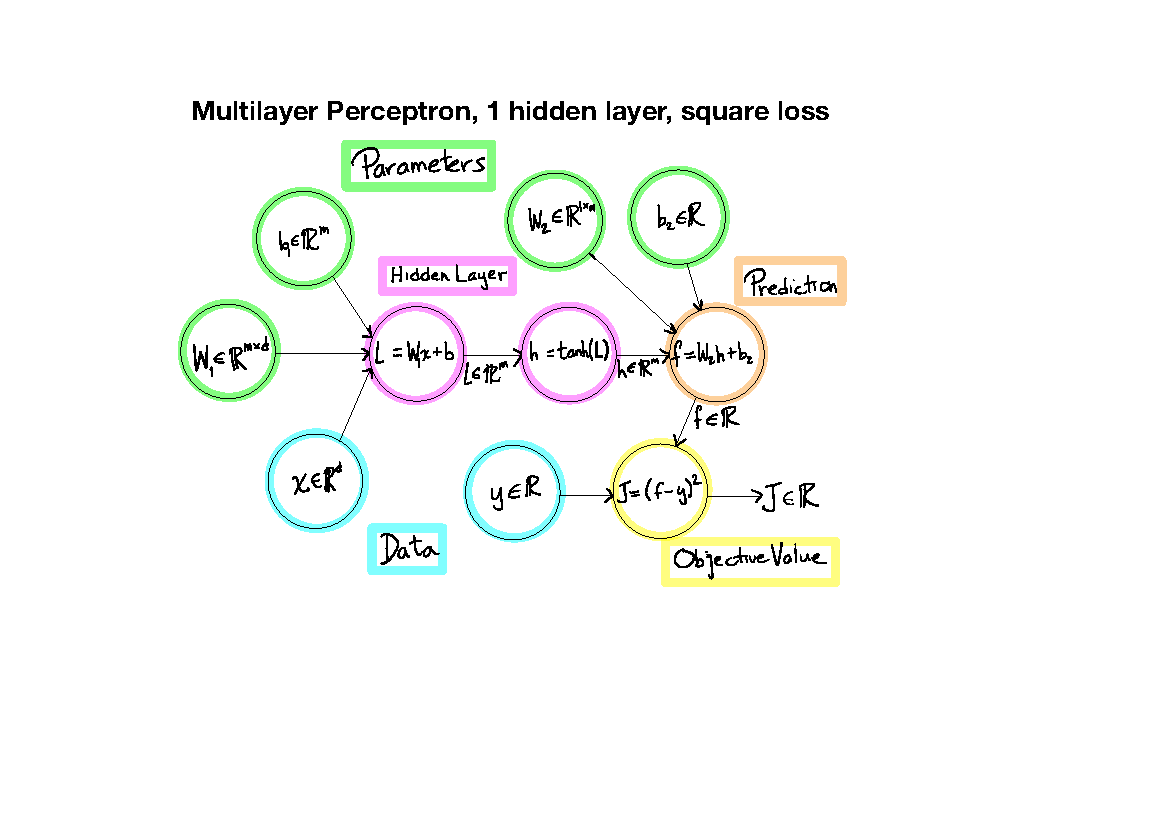
\includegraphics{MLP-computation-graph}
\par\end{center}

The crucial new piece here is the nonlinear \textbf{hidden layer},
which is what makes the multilayer perceptron a significantly larger
hypothesis space than linear prediction functions.

\subsection{The standard non-linear layer}

The multilayer perceptron consists of a sequence of ``layers'' implementing
the following non-linear function
\[
h(x)=\sigma\left(Wx+b\right),
\]
where $x\in\reals^{d}$, $W\in\reals^{m\times d},$ and $b\in\reals^{m}$,
and where $m$ is often referred to as the number of\textbf{ hidden
units }or\textbf{ hidden nodes}. $\sigma$ is some non-linear function,
typically $\tanh$ or ReLU, applied element-wise to the argument of
$\sigma$. Referring to the computation graph illustration above,
we will implement this nonlinear layer with two nodes, one implementing
the affine transform $L=W_{1}x+b_{1}$, and the other implementing
the nonlinear function $h=\tanh(L)$. In this problem, we'll work
out how to implement the backward method for each of these nodes.

\subsubsection{The Affine Transformation}

In a general neural network, there may be quite a lot of computation
between any given affine transformation $Wx+b$ and the final objective
function value $J$. We will capture all of that in a function $f:\reals^{m}\to\reals$,
for which $J=f(Wx+b)$. Our goal is to find the partial derivative
of $J$ with respect to each element of $W$, namely $\partial J/\partial W_{ij}$,
as well as the partials $\partial J/\partial b_{i}$, for each element
of $b$. For convenience, let $y=Wx+b$, so we can write $J=f(y)$.
Suppose we have already computed the partial derivatives of $J$ with
respect to the entries of $y=\left(y_{1},\ldots,y_{m}\right)^{T}$,
namely $\frac{\partial J}{\partial y_{i}}$ for $i=1,\ldots,m$. Then
by the chain rule, we have
\[
\frac{\partial J}{\partial W_{ij}}=\sum_{r=1}^{m}\frac{\partial J}{\partial y_{r}}\frac{\partial y_{r}}{\partial W_{ij}}.
\]

\begin{enumerate}
\item Show that $\frac{\partial J}{\partial W_{ij}}=\frac{\partial J}{\partial y_{i}}x_{j}$,
where $x=\left(x_{1},\ldots,x_{d}\right)^{T}$. {[}Hint: Although
not necessary, you might find it helpful to use the notation $\delta_{ij}=\begin{cases}
1 & i=j\\
0 & \text{else}
\end{cases}$. So, for examples, $\partial_{x_{j}}\left(\sum_{i=1}^{n}x_{i}^{2}\right)=2x_{i}\delta_{ij}=2x_{j}$.{]}


\item Now let's vectorize this. Let's write $\frac{\partial J}{\partial y}\in\reals^{m\times1}$
for the column vector whose $i$th entry is $\frac{\partial J}{\partial y_{i}}$.
Let's also define the matrix $\frac{\partial J}{\partial W}\in\reals^{m\times d}$,
whose $ij$'th entry is $\frac{\partial J}{\partial W_{ij}}$. Generally
speaking, we'll always take $\frac{\partial J}{\partial A}$ to be
an array of the same size (``shape'' in numpy) as $A$. Give a vectorized
expression for $\frac{\partial J}{\partial W}$ in terms of the column
vectors $\frac{\partial J}{\partial y}$ and $x$. {[}Hint: Outer
product.{]}

\item In the usual way, define $\frac{\partial J}{\partial x}\in\reals^{d}$,
whose $i$'th entry is $\frac{\partial J}{\partial x_{i}}$. Show
that 
\[
\frac{\partial J}{\partial x}=W^{T}\left(\frac{\partial J}{\partial y}\right)
\]
{[}Note, if $x$ is just data, technically we won't need this derivative.
However, in a multilayer perceptron, $x$ may actually be the output
of a previous hidden layer, in which case we will need to propagate
the derivative through $x$ as well.{]} \\


\item Show that $\frac{\partial J}{\partial b}=\frac{\partial J}{\partial y}$,
where $\frac{\partial J}{\partial b}$ is defined in the usual way.

\end{enumerate}


\subsubsection{Element-wise Transformers}

Our nonlinear activation function nodes take an array (e.g. a vector,
matrix, higher-order tensor, etc), and apply the same nonlinear transformation
$\sigma:\reals\to\reals$ to every element of the array. Let's abuse
notation a bit, as is usually done in this context, and write $\sigma(A)$
for the array that results from applying $\sigma(\cdot)$ to each
element of $A$. If $\sigma$ is differentiable at $x\in\reals$,
then we'll write $\sigma'(x)$ for the derivative of $\sigma$ at
$x$, with $\sigma'(A)$ defined analogously to $\sigma(A)$.

Suppose the objective function value $J$ is written as $J=f(\sigma(A))$,
for some function $f:S\mapsto\reals$, where $S$ is an array of the
same dimensions as $\sigma(A)$ and $A$. As before, we want to find
the array $\frac{\partial J}{\partial A}$ for any $A$. Suppose for
some $A$ we have already computed the array $\frac{\partial J}{\partial S}=\frac{\partial f(S)}{\partial S}$
for $S=\sigma(A)$. At this point, we'll want to use the chain rule
to figure out $\frac{\partial J}{\partial A}$. However, because we're
dealing with arrays of arbitrary shapes, it can be tricky to write
down the chain rule. Appropriately, we'll use a tricky convention:
We'll assume all entries of an array $A$ are indexed by a single
variable. So, for example, to sum over all entries of an array $A$,
we'll just write $\sum_{i}A_{i}$. 
\begin{enumerate}
\item Show that $\frac{\partial J}{\partial A}=\frac{\partial J}{\partial S}\odot\sigma'(A)$,
where we're using $\odot$ to represent the \textbf{Hadamard product}.
If $A$ and $B$ are arrays of the same shape, then their Hadamard
product $A\odot B$ is an array with the same shape as $A$ and $B$,
and for which $\left(A\odot B\right)_{i}=A_{i}B_{i}$. That is, it's
just the array formed by multiplying corresponding elements of $A$
and $B$. Conveniently, in \code{numpy} if \code{A} and \code{B}
are arrays of the same shape, then \code{A{*}B} is their Hadamard
product. 

\end{enumerate}

\subsection{MLP Implementation}
\begin{enumerate}
\item Complete the class \code{AffineNode} in \code{nodes.py}. Be sure
to propagate the gradient with respect to $x$ as well, since when
we stack these layers, $x$ will itself be the output of another node
that depends on our optimization parameters.
\item Complete the class \code{TanhNode} in \code{nodes.py}. As you'll
recall, $\frac{d}{dx}\tanh(x)=1-\tanh^{2}x$. Note that in the forward
pass, we'll already have computed $\tanh$ of the input and stored
it in self.out. So make sure to use \code{self.out} and not recalculate
it in the backward pass.
\item Implement an MLP by completing the skeleton code in \code{mlp\_regression.py}
and making use of the nodes above. Your code should pass the tests
provided in \code{mlp\_regression.t.py}. Note that to break the symmetry
of the problem, we initialize our weights to small random values,
rather than all zeros, as we often do for convex optimization problems.
Run the MLP for the two settings given in the \code{main()} function
and report the average \textbf{training} error. Note that with an
MLP, we can take the original scalar as input, in the hopes that it
will learn nonlinear features on its own, using the hidden layers.
In practice, it is quite challenging to get such a neural network
to fit as well as one where we provide features. 
\item {[}Optional{]} See if you can get a fit on the training set with an
MLP that uses just the scalar input that is about as good as the fit
using the featurized inputs. You can do that by tweaking model parameters
(e.g. the number of hidden nodes or layers) and/or the parameters
of optimization. You \textbf{may use} any neural network framework
(PyTorch, TensorFlow, etc), which can help by providing more advanced
optimization techniques (e.g. Adam), variable initialization methods,
and/or various normalization approaches (batch norm, etc). 
\end{enumerate}

\subsection{{[}OPTIONAL{]}}
\begin{enumerate}
\item {[}Optional{]} Implement a Softmax node.
\item {[}Optional{]} Implement a negative log-likelihood loss node for multiclass
classification.
\item {[}Optional{]} Use the classes above to apply an MLP to the simple
multiclass classification dataset we had on a previous assignment.
\end{enumerate}

\end{document}